\documentclass[../../syllabus_2.tex]{subfiles}
\begin{document}
\chapter{Proportionnalité et projections parallèles} 

\section{Tableau de proportionnalité}

%\begin{exercise} 
Pour son anniversaire, Diego reçoit un smartphone. Il lui reste à choisir un abonnement. Il se rend chez un opérateur qui lui propose deux tarifs: le tarif standard à 0,50€/minute d'appel et SMS illimités ou le tarif premium à 10€ fixe et 0,25€ / minutute d'appel et SMS illimités. 
\begin{enumerate}
    \item Pour chaque tarif, établis un tableau:
    Tarif standard:
    \begin{center}
        \begin{tblr}{hlines, vlines, columns={c}, rows={m},column{1}={5cm,l}}
            Minutes appelées & 0 & 5 & 10 & 15 & 20 & 25 & 30 & 35 \\
            Prix à payer en € &  &   &    &    &    &    &    &    
        \end{tblr}
    \end{center}

    Tarif premium:
    \begin{center}
        \begin{tblr}{hlines, vlines, columns={c}, rows={m},column{1}={5cm,l}}
            Minutes appelées & 0 & 5 & 10 & 15 & 20 & 25 & 30 & 35 \\
            Prix à payer en € &  &   &    &    &    &    &    &    
        \end{tblr}
    \end{center}
    
    \item Représente graphiquement ces deux tarifs ci-dessous.     
    \begin{center}
        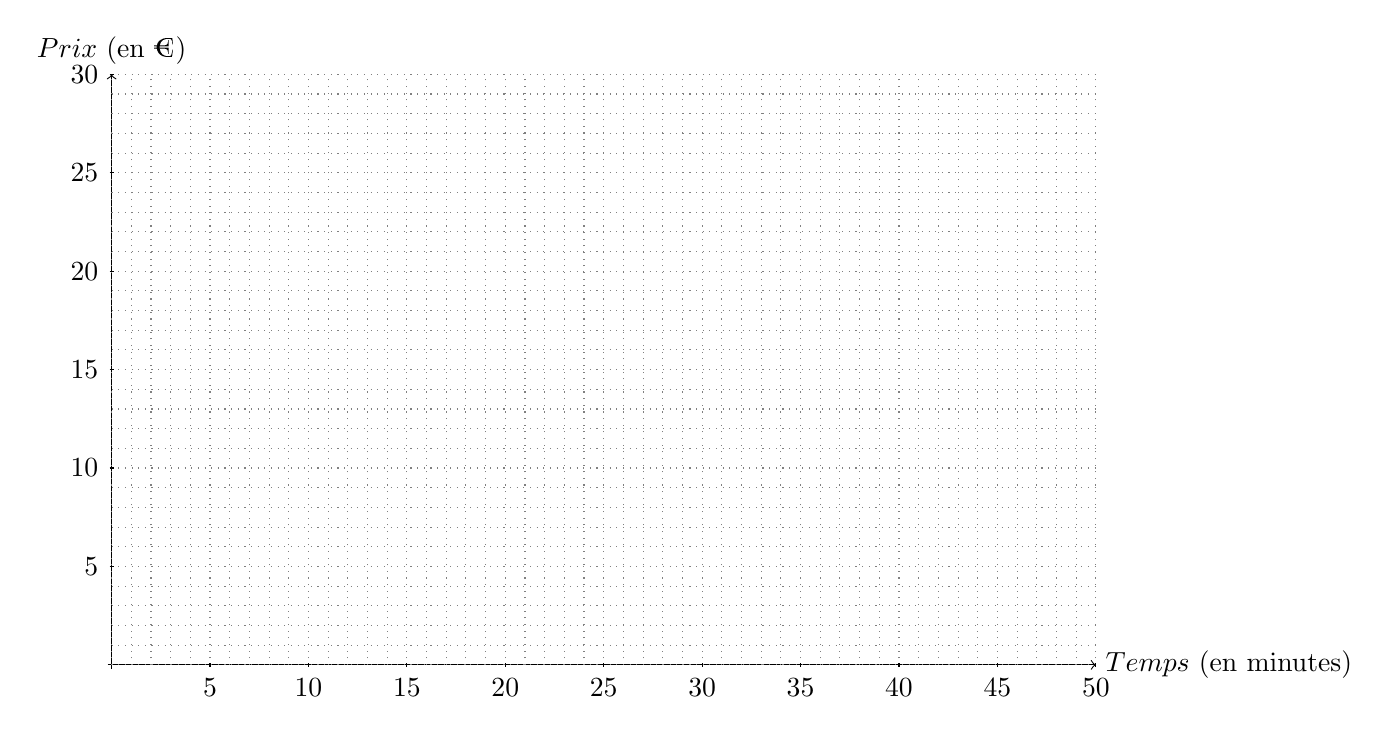
\begin{tikzpicture}[scale=0.25]
            % Axes
            \draw[->] (0,-0.20) -- (0,30) node[above] {$Prix$ (en €)};
            \draw[->] (-0.20,0) -- (50,0) node[right] {$Temps$ (en minutes)};
            % Grille
            \draw[gray, dotted] (0,0) grid (50,30);
            % Graduations
            \foreach \x in {5,10,15,20,25,30,35,40,45,50}
                \draw (\x,-0.1) -- (\x,0.1) node[below=2pt] {\x};
            \foreach \y in {5,10,15,20,25,30}
                \draw (-0.1,\y) -- (0.1,\y) node[left=2pt] {\y};
        \end{tikzpicture}
    \end{center}
    
    \item Ces deux tarifs représentent-ils des relations directement proportionnelles ? Justifie.
    \adf{2}

\hskip -20pt
\adf[\textbf{Définition:} Deux grandeurs sont proportionnelles si ]{3} 
%on obtient la seconde grandeur en multipliant la première par un nombre constant. Ce nombre est appelé le coefficient de proportionnalité et est noté k.


    \item Si on pose x le nombre de minutes et y le prix en €, écrit la relation qui unit ces deux valeurs. 
    \adf{1}

    \item Dans cet exemple, le coefficient de proportionnalité vaut :

\hskip -20pt
Formule générale
    \begin{center}
    $ y = k \cdot x$
    \end{center}
    
    \begin{center}
    k = coefficient de proportionnalité = $\dfrac{y}{x}= \dfrac{seconde grandeur}{permière grandeur}$
    \end{center}

    \item Comment peut-on reconnaitre graphiquement qu'il s'agit d'une relation directement proportionnelle ? 
    \adf{2}
\end{enumerate}
%\end{exercise}

Ainsi, lorsque nous nous retrouvons face à un tableau, nous pouvons déterminer le coefficient de proportionnalité en divisant la valeur dépendante par la valeur indépendante. 
\begin{exercise}
    Complète les tableaux suivants pour qu'ils correspondent à des situations de proportionnalitédirecte et indique le coefficient de proportionnalité k pour passer de x à y.
    \begin{enumerate}
        \item k = 
        \newline
        \begin{tblr}{hlines, vlines, columns={c}, rows={m}}
            x & 5 & 8  & 10 & 16 \\
            y &   & 48 & 66 &        
        \end{tblr}
        \item k =
        \newline
        \begin{tblr}{hlines, vlines, columns={c}, rows={m}}
            x & 5 & 8  & 10 & 16 \\
            y &   & 48 & 66 &        
        \end{tblr}
        \item k =
        \newline
        \begin{tblr}{hlines, vlines, columns={c}, rows={m}}
            x & 5 & 8  & 10 & 16 \\
            y &   & 48 & 66 &        
        \end{tblr}
    \end{enumerate}
\end{exercise}

%\begin{exercise}
    Cristina et Elena, deux amies, vont à l'école à vélo. Elles partent au même moment de leur immeuble mais ne font pas le trajet ensemble. Voici les données pour un matin du mois de mai.

    Pour Cristina:
    \begin{center}
        \begin{tblr}{hlines, vlines, columns={c}, rows={m},column{1}={5cm,l}}
            Temps de trajet (minutes) & 0 & 5 & 10 & 15 & 20 & 25 & 30 \\
            Distance parcourue (km) & 0 & 1,25 & 2,5 & 3,75 & 5 & 6,25  & 7,5       
        \end{tblr}
    \end{center}

    Pour Elena, elle est arrivée en retard, voici ce qu'elle explique à son éducateur: \textit{"Je sais qu'il est 08h45 Monsieur, mais je n'ai pas eu de chance ce matin. Je suis partie de chez moi à 7h50, au début j'allais à mon aise (10km/h). A 8h05, je me suis arretée pour attendre Batuhan. Il est arrivé à 8h10, et comme on était déjà un peu en retard, on a acceléré (15km/h). Malheureusement, à 08h20 j'ai roulé sur un clou et j'ai crevé mon pneu. On a essayé de le réparer pendant 10 minutes mais ça n'a pas marché. Je suis donc montée sur le porte-baggage de Batuhan, et il a pédalé pour deux. C'était plus dur (10km/h). On est désolé Monsieur, on a fait de notre mieux".}

    \begin{enumerate}
        \item Complète le tableau de valeurs pour le trajet d'Elena.
        \begin{center}
            \begin{tblr}{hlines, vlines, columns={c}, rows={m},column{1}={5cm,l}}
                Temps de trajet (minutes) & 0 & 5 & 10 & 15 & 20 & 25 & 30 \\
                Distance parcourue (km)   &   &   &    &    &    &    &        
            \end{tblr}
        \end{center}
        \item Trace le graphique qui représente le trajet d'Elena ainsi que celui de Cristina. Utilise des couleurs différentes. 
        \begin{center}
            \begin{tikzpicture}[scale=1.1]
                % Axes
                \draw[->] (0,-0.20) -- (0,10) node[above] {$Distance parcourue$ (km)};
                \draw[->] (-0.20,0) -- (10,0) node[right] {$Temps$ (heure)};
                % Grille
                \draw[gray, dotted] (0,0) grid (10,10);
                % Graduations
                \foreach \x in {} %mettre les heures 7h50 - 8h50
                    \draw (\x,-0.1) -- (\x,0.1) node[below=2pt] {\x};
                \foreach \y in {,1,2,3,4,5,6,7,8,9}
                    \draw (-0.1,\y) -- (0.1,\y) node[left=2pt] {\y};
            \end{tikzpicture}
        \end{center}
        \item Quel graphique représente une relation proportionnelle entre distance et temps? 
        \adf{2}
        \item Quel est le coefficient de proportionnalité pour ce graphique ?
        \adf{2}
    \end{enumerate}

%\end{exercise}

\section{Propriété fondamentale des proportions}
Comme vu dans le chapitre sur les équations, lorsque nous avons une égalité de deux fractions $\dfrac{a}{b}=\dfrac{c}{d}$ nous pouvons la réécrire comme $a\cdot d = b \cdot c$.
Ecris toutes les autres égalités possibles à partir de cette égalité $\dfrac{a}{b}=\dfrac{c}{d}$ si a, b,c et d sont différents de 0. 

\adf[\textbf{Définition:} Une proportion est une égalité entre deux rapports.]{2}

Dans la proportion $\dfrac{a}{b}=\dfrac{c}{d}$ 
a, b, c et d sont les termes,
a et d sont les extrèmes et
b et c sont les moyens. 

\adf[\textbf{Propriété fondamentale:} Dans toute proportion, le produit des extrêmes est égal au produit des moyens.]{2}


\begin{exercise}
    Nathan et Samuel veulent repeindre le local de leur classe en vert clair. Pour obtenir cette couleur, il faut mélanger du bleu et de jaune. Nathan a estimé qu'il fallait une portion de bleu pour cinq de jaune. Il effectue le mélange. A ce moment-là Samuel arrive et lui dit "C'est beaucoup trop clair, il fallait faire le contraire: cinq portions de bleu et une de jaune". Combien Nathan doit-il rajouter de portions de bleu pour obtenir la bonne couleur ?
\end{exercise}

\begin{exercise}
    Exercice fast-food
\end{exercise}

\section{Projections parallèles}

Mise en situation avec les ombres

\section{Agrandissement et réduction}

A partir des exemples précendents, complète la synthèse suivante.
\textbf{Synthèse}
Les agrandissements et les réductions conservent:
\begin{itemize}[label=$\bullet$]
    \item La forme des figures
    \item L'amplitude des angles
    \item Le parallélisme et la perpendicularité
\end{itemize}

Dans un agrandissement ou une réduction, les côtés homologues ont des longeurs proportionnelles:
\begin{itemize}[label=$\bullet$]
    \item Pour un agrandissement: k > 1
    \item Pour une réduction: k < 1
    \item Pour une isométrie : k = 1
\end{itemize}

\section{Exercices mélangés}

\end{document}